\documentclass[border=2pt]{standalone}
\usepackage{pgfplots}
\begin{document}
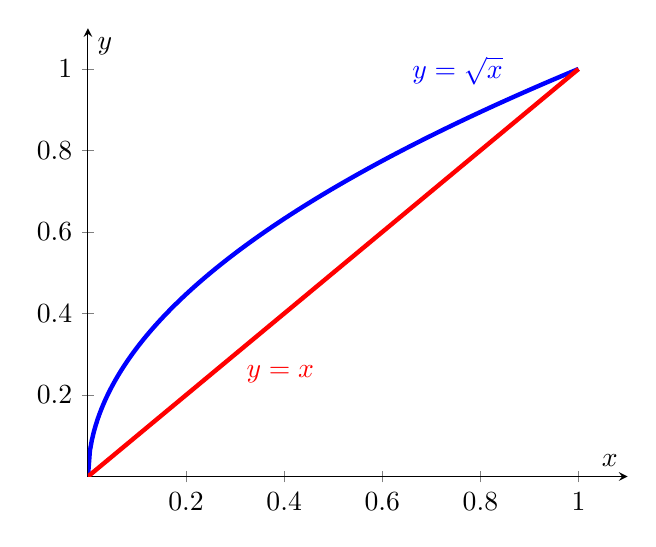
\begin{tikzpicture}
  \begin{axis}[
      axis lines=center,        % so that origin is at 0,0
      xmax = 1.1,
      ymax = 1.1,
      ylabel=$y$,
      xlabel=$x$,
    ]
    \addplot [domain=0:1,samples=250, ultra thick, blue] {sqrt(x)}
    node [pos=0.9, above left] {$y=\sqrt{x}$}; % pos is pos along curve
    \addplot [domain=0:1,samples=250, ultra thick, red ] {x}
    node [pos=0.3, below right] {$y=x$};
  \end{axis}
\end{tikzpicture}
\end{document}
